\documentclass[a4paper, twoside=true, 12pt]{extreport}
% basics
\usepackage[utf8]{inputenc}
\usepackage[T1]{fontenc}
\usepackage{textcomp}
% \usepackage[dutch]{babel}
\usepackage{url}
\usepackage{hyperref}
\hypersetup{colorlinks=true, pdfstartview=FitV, linkcolor=blue, 
citecolor=black, plainpages=false, urlcolor=black}
\usepackage{graphicx}
\usepackage{float}
\usepackage{booktabs}
\usepackage{enumitem}
\usepackage{parskip}
\usepackage{emptypage}
\usepackage{subcaption}
\usepackage{multicol}
\usepackage{cprotect}
\usepackage{multirow}
\usepackage{verbatimbox}
\usepackage{listings}
\usepackage{xparse}
\usepackage{multirow}
\usepackage[usenames,dvipsnames]{xcolor}

% \usepackage{cmbright}
\usepackage{geometry}
\geometry{a4paper, twoside=true}
\geometry{
 a4paper,
 total={170mm,257mm},
 left=25mm,
 top=20mm, 
 right = 25mm
 }


\usepackage{amsmath, amsfonts, mathtools, amsthm, amssymb}
\usepackage{mathrsfs}
\usepackage{cancel}
\usepackage{bm}
\newcommand\N{\ensuremath{\mathbb{N}}}
\newcommand\R{\ensuremath{\mathbb{R}}}
\newcommand\Z{\ensuremath{\mathbb{Z}}}
\renewcommand\O{\ensuremath{\emptyset}}
\newcommand\Q{\ensuremath{\mathbb{Q}}}
\newcommand\C{\ensuremath{\mathbb{C}}}
\DeclareMathOperator{\sgn}{sgn}
\usepackage{systeme}
\let\svlim\lim\def\lim{\svlim\limits}
\let\implies\Rightarrow
\let\impliedby\Leftarrow
\let\iff\Leftrightarrow
\let\epsilon\varepsilon
\usepackage{stmaryrd} % for \lightning
\newcommand\contra{\scalebox{1.1}{$\lightning$}}
% \let\phi\varphi

\usepackage{titlesec}

\titleformat{\chapter}[hang] 
{\normalfont \fontsize{20pt}{40pt}\bfseries}{\thechapter.}{0.55em}{}   
\titlespacing{\chapter}{0pt}{-30pt}{3px}

\titleformat{\section}[hang]
{\normalfont \fontsize{18px}{18px}\bfseries}{\thesection}{1em}{}
\titlespacing{\section}{0px}{20px}{15px}





% correct
\definecolor{correct}{HTML}{009900}
\newcommand\correct[2]{\ensuremath{\:}{\color{red}{#1}}\ensuremath{\to }{\color{correct}{#2}}\ensuremath{\:}}
\newcommand\green[1]{{\color{correct}{#1}}}



% horizontal rule
\newcommand\hr{
    \noindent\rule[0.5ex]{\linewidth}{0.5pt}
}


% hide parts
\newcommand\hide[1]{}



% si unitx
\usepackage{siunitx}
\sisetup{locale = UK}
% \renewcommand\vec[1]{\mathbf{#1}}
\newcommand\mat[1]{\mathbf{#1}}


% tikz
\usepackage{tikz}
\usepackage{tikz-cd}
\usetikzlibrary{intersections, angles, quotes, calc, positioning}
\usetikzlibrary{arrows.meta}
\usepackage{pgfplots}
\pgfplotsset{compat=1.13}


\tikzset{
    force/.style={thick, {Circle[length=2pt]}-stealth, shorten <=-1pt}
}

% theorems
\makeatother
\usepackage{thmtools}
\usepackage[framemethod=TikZ]{mdframed}
\mdfsetup{skipabove=1em,skipbelow=0em}


\theoremstyle{definition}

\declaretheoremstyle[
    headfont=\bfseries\sffamily\color{ForestGreen!70!black}, bodyfont=\normalfont,
    mdframed={
        linewidth=2pt,
        rightline=false, topline=false, bottomline=false,
        linecolor=ForestGreen, backgroundcolor=ForestGreen!5,
    }
]{thmgreenbox}

\declaretheoremstyle[
    headfont=\bfseries\sffamily\color{NavyBlue!70!black}, bodyfont=\normalfont,
    mdframed={
        linewidth=2pt,
        rightline=false, topline=false, bottomline=false,
        linecolor=NavyBlue, backgroundcolor=NavyBlue!5,
    }
]{thmbluebox}

\declaretheoremstyle[
    headfont=\bfseries\sffamily\color{NavyBlue!70!black}, bodyfont=\normalfont,
    mdframed={
        linewidth=2pt,
        rightline=false, topline=false, bottomline=false,
        linecolor=NavyBlue
    }
]{thmblueline}

\declaretheoremstyle[
    headfont=\bfseries\sffamily\color{RawSienna!70!black}, bodyfont=\normalfont,
    mdframed={
        linewidth=2pt,
        rightline=false, topline=false, bottomline=false,
        linecolor=RawSienna, backgroundcolor=RawSienna!5,
    }
]{thmredbox}

\declaretheoremstyle[
    headfont=\bfseries\sffamily\color{RawSienna!70!black}, bodyfont=\normalfont,
    numbered=no,
    mdframed={
        linewidth=2pt,
        rightline=false, topline=false, bottomline=false,
        linecolor=RawSienna, backgroundcolor=RawSienna!1,
    },
    qed=\qedsymbol
]{thmproofbox}

\declaretheoremstyle[
    headfont=\bfseries\sffamily\color{NavyBlue!70!black}, bodyfont=\normalfont,
    numbered=no,
    mdframed={
        linewidth=2pt,
        rightline=false, topline=false, bottomline=false,
        linecolor=NavyBlue, backgroundcolor=NavyBlue!1,
    },
]{thmexplanationbox}



% \declaretheoremstyle[headfont=\bfseries\sffamily, bodyfont=\normalfont, mdframed={ nobreak } ]{thmgreenbox}
% \declaretheoremstyle[headfont=\bfseries\sffamily, bodyfont=\normalfont, mdframed={ nobreak } ]{thmredbox}
% \declaretheoremstyle[headfont=\bfseries\sffamily, bodyfont=\normalfont]{thmbluebox}
% \declaretheoremstyle[headfont=\bfseries\sffamily, bodyfont=\normalfont]{thmblueline}
% \declaretheoremstyle[headfont=\bfseries\sffamily, bodyfont=\normalfont, numbered=no, mdframed={ rightline=false, topline=false, bottomline=false, }, qed=\qedsymbol ]{thmproofbox}
% \declaretheoremstyle[headfont=\bfseries\sffamily, bodyfont=\normalfont, numbered=no, mdframed={ nobreak, rightline=false, topline=false, bottomline=false } ]{thmexplanationbox}

\declaretheorem[style=thmgreenbox, name=Definition]{definition}
\declaretheorem[style=thmbluebox, numbered=no, name=Example]{eg}
\declaretheorem[style=thmredbox, name=Proposition]{prop}
\declaretheorem[style=thmredbox, name=Theorem]{theorem}
\declaretheorem[style=thmredbox, name=Lemma]{lemma}
\declaretheorem[style=thmredbox, numbered=no, name=Corollary]{corollary}

\declaretheorem[style=thmproofbox, name=Proof]{replacementproof}
\renewenvironment{proof}[1][\proofname]{\vspace{-10pt}\begin{replacementproof}}{\end{replacementproof}}


\declaretheorem[style=thmexplanationbox, name=Proof]{tmpexplanation}
\newenvironment{explanation}[1][]{\vspace{-10pt}\begin{tmpexplanation}}{\end{tmpexplanation}}

\declaretheorem[style=thmblueline, numbered=no, name=Remark]{remark}
\declaretheorem[style=thmblueline, numbered=no, name=Note]{note}

\newtheorem*{uovt}{UOVT}
\newtheorem*{notation}{Notation}
\newtheorem*{previouslyseen}{As previously seen}
\newtheorem*{problem}{Problem}
\newtheorem*{observe}{Observe}
\newtheorem*{property}{Property}
\newtheorem*{intuition}{Intuition}


\usepackage{etoolbox}
\AtEndEnvironment{vb}{\null\hfill$\diamond$}%
\AtEndEnvironment{intermezzo}{\null\hfill$\diamond$}%
% \AtEndEnvironment{opmerking}{\null\hfill$\diamond$}%

% http://tex.stackexchange.com/questions/22119/how-can-i-change-the-spacing-before-theorems-with-amsthm
\makeatletter
% \def\thm@space@setup{%
%   \thm@preskip=\parskip \thm@postskip=0pt
% }

\newcommand{\oefening}[1]{%
    \def\@oefening{#1}%
    \subsection*{Oefening #1}
}

\newcommand{\suboefening}[1]{%
    \subsubsection*{Oefening \@oefening.#1}
}

\newcommand{\exercise}[1]{%
    \def\@exercise{#1}%
    \subsection*{Exercise #1}
}

\newcommand{\subexercise}[1]{%
    \subsubsection*{Exercise \@exercise.#1}
}


\usepackage{xifthen}

\def\testdateparts#1{\dateparts#1\relax}
\def\dateparts#1 #2 #3 #4 #5\relax{
    \marginpar{\small\textsf{\mbox{#1 #2 #3 #5}}}
}

\def\@lesson{}%
\newcommand{\lesson}[3]{
    \ifthenelse{\isempty{#3}}{%
        \def\@lesson{Chapter #1}%
    }{%
        \def\@lesson{Chapter #1: #3}%
    }%
   % \subsection*{\@lesson}
  %\testdateparts{#2}
}

% \renewcommand\date[1]{\marginpar{#1}}


% fancy headers
\usepackage{fancyhdr}
\pagestyle{fancy}

% \fancyhead[LE,RO]{Gilles Castel}
\fancyhead[RO,LE]{\@lesson}
\fancyhead[RE,LO]{}
\fancyfoot[LE,RO]{\thepage}
\fancyfoot[C]{\leftmark}

\makeatother



\setlength {\marginparwidth }{2cm} 
% notes
\usepackage{todonotes}
\usepackage{tcolorbox}

\tcbuselibrary{breakable}
\newenvironment{verbetering}{\begin{tcolorbox}[
    arc=0mm,
    colback=white,
    colframe=green!60!black,
    title=Opmerking,
    fonttitle=\sffamily,
    breakable
]}{\end{tcolorbox}}

\newenvironment{noot}[1]{\begin{tcolorbox}[
    arc=0mm,
    colback=white,
    colframe=white!60!black,
    title=#1,
    fonttitle=\sffamily,
    breakable
]}{\end{tcolorbox}}




% figure support
\usepackage{import}
\usepackage{xifthen}
\pdfminorversion=7
\usepackage{pdfpages}
\usepackage{transparent}
\newcommand{\incfig}[1]{%
    \def\svgwidth{\columnwidth}
    \import{./figures/}{#1.pdf_tex}
}

% %http://tex.stackexchange.com/questions/76273/multiple-pdfs-with-page-group-included-in-a-single-page-warning
\pdfsuppresswarningpagegroup=1


\author{Akash Gopinath}


%%%%%
% another center environment that does not add whitespace
\newenvironment{mycenter}[1][\topsep]
  {\setlength{\topsep}{#1}\par\kern\topsep\centering}% \begin{mycenter}[<len>]
  {\par\kern\topsep}% \end{mycenter}
  %%%%%
  
%%%%%
% another flushright environment that does not add whitespace
  \newenvironment{myright}[1][\topsep]
  {\setlength{\topsep}{#1}\par\kern\topsep\raggedleft}% \begin{myright}[<len>]
  {\par\kern\topsep}% \end{myright}

%%%%%%%%%%%%%%%%%%%%%%%%%%%%%%%%%%%%%%%%%%%%%%%%%%%%%%%%%%%%%%%%%%%%%%%%%
  \newenvironment{myleft}[1][\topsep]
  {\setlength{\topsep}{#1}\par\kern\topsep\raggedright}% \begin{myright}[<len>]
  {\par\kern\topsep}% \end{myright}
%%%%%%%%%%%%%%%%%%%%%%%%%%%%%%%%%%%%%%%%%%%%%%%%%%%%%%%%%%%%%%%%%%%%%%%%%


\DeclareMathOperator{\length}{length}
\DeclareMathOperator{\Aut}{Aut}
\DeclareMathOperator{\diam}{diam}
\DeclareMathOperator*{\res}{res}

\usepackage{faktor}

\makeatletter
\DeclareRobustCommand*{\mfaktor}[3][]
{
   { \mathpalette{\mfaktor@impl@}{{#1}{#2}{#3}} }
}
\newcommand*{\mfaktor@impl@}[2]{\mfaktor@impl#1#2}
\newcommand*{\mfaktor@impl}[4]{
   \settoheight{\faktor@zaehlerhoehe}{\ensuremath{#1#2{#3}}}%
   \settoheight{\faktor@nennerhoehe}{\ensuremath{#1#2{#4}}}%
      \raisebox{-0.5\faktor@zaehlerhoehe}{\ensuremath{#1#2{#3}}}%
      \mkern-4mu\diagdown\mkern-5mu%
      \raisebox{0.5\faktor@nennerhoehe}{\ensuremath{#1#2{#4}}}%
}
\makeatother

\title{Vector and Complex Calculus}

\begin{document}
    \maketitle
    \tableofcontents
    \clearpage
     % start lectures
     \lesson{1}{2023-10-16 20:17}{Vectors}
\chapter{Vectors}

\section{Introduction}

\begin{definition}[Vectors]
  Vectors are mathematical objects with both {\bf magnitude} and {\bf direction}.
\end{definition}
Geometrially, vectors can be thought of as arrows/direced line segments in space in space.
\begin{figure}[H]
\centering
   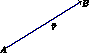
\includegraphics[scale=3.0]{vector.pdf}
   \caption{A Vector}
   \label{fig:figure-1-vector}
\end{figure}


\begin{eg}[Examples of vectors]
  Here are some important examples of vectors\\
  \vspace{-10px}
  \begin{itemize}
    \item The displacement of a particle is a vector.
    \item The velocity of a particle is a vector.
    \item The force acting on a particle is a vector.
  \end{itemize}

\end{eg}

\begin{notation}
  Vectors can be denoted in 3 ways,
  \begin{itemize}
    \item Using {\bf boldface notation}: $\boldsymbol{V}$
    \item Underlining:  $\underline{V}$ 
    \item An arrow over the symbol: $\vec{V}$

  \end{itemize}


\end{notation}

\section{Euclidean Three Space $\mathbb{E}^3$}

\begin{definition}[Euclidian Three Space]
 
  Euclidean Three Space is the set of all ordered triples of real numbers.\\
  \vspace{-10px}
  \begin{equation}
    \mathbb{E}^3 = \{(x,y,z) | x,y,z \in \mathbb{R}\}
  \end{equation}

\end{definition}

The \textbf{axes} of $\mathbb{E}^{3}$ are the $x$, $y$ and $z$, i.e.
\vspace{-10px}
\begin{equation}
  x = (x,0,0), y = (0,y,0), z = (0,0,z)
\end{equation}

We orient the axis according to the \textbf{right hand rule}. This is shown in the following diagram:

%generate tikz code for axes in 3d space

\begin{figure}[H]
  \centering
  \begin{tikzpicture}
    \draw[->] (0,0,0) -- (3,0,0) node[anchor=north east]{$y$};
    \draw[->] (0,0,0) -- (0,3,0) node[anchor=north west]{$z$};
    \draw[->] (0,0,0) -- (0,0,3) node[anchor=south]{$x$};
  \end{tikzpicture}
  \caption{Axes in $\mathbb{E}^3$}
\end{figure}

\begin{note}
  We need to pick an \textbf{origin} and stay with it. We will use the origin $(0,0,0)$.
\end{note} 

\section{Vectors in $\mathbb{E}^3$}
\subsection{Distance in $\mathbb{E}^3$}
Let $P$ and $P^{'}$ be points in $\mathbb{E}^3$. And let $P = (x,y,z)$ and $P^{'} = (x^{'},y^{'},z^{'})$.
\begin{definition}[Distance in $\mathbb{E}^3$]
  The \textbf{distance} between $P$ and $P^{'}$ is defined as:
  \begin{equation}
    d(P,P^{'}) = \sqrt{(x-x^{'})^2 + (y-y^{'})^2 + (z-z^{'})^2}
  \end{equation}
\end{definition}
This is illustrated in the following diagram
\begin{figure}[H]
\centering
   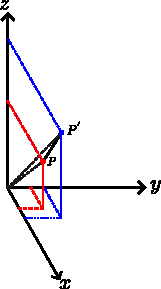
\includegraphics[scale=1.75]{distance.pdf}
   \caption{Distance in $\mathbb{E}^3$}
   \label{fig:figure-8-space}
\end{figure}
\clearpage
\subsection{Vectors in $\mathbb{E}^3$}
\begin{definition}[Vectors in $\mathbb{E}^3$]
  A \textbf{vector} in $\mathbb{E}^3$ is an ordered triple of real numbers.\\
  \vspace{-10px}
  \begin{equation}
    \vec{v} = (v_1,v_2,v_3)
  \end{equation}
\end{definition}

\begin{notation}
  We can also represent vectors using {\bf column notation}
  $$\underline{v} = \begin{bmatrix} v_1 \\ v_2 \\ v_3\end{bmatrix} $$
  
\end{notation}


     \section{Vector Algebra}

\subsection{Vector Magnitude}

\begin{definition}[Vector Magnitude]
  Let $\vec{v} = (v_1, v_2, v_3)$ be a vector in $\mathbb{E}^3$. The \textbf{magnitude} of $\vec{v}$ is defined as:
  \begin{equation}
    \|\vec{v}\| = \sqrt{v_1^2 + v_2^2 + v_3^2}
  \end{equation}
\end{definition}

\subsection{Vector Addition}

\begin{definition}[Vector Addition]
  Let $\vec{v} = (v_1, v_2, v_3)$ and $\vec{w} = (w_1, w_2, w_3)$ be vectors in $\mathbb{E}^3$. The \textbf{sum} of $\vec{v}$ and $\vec{w}$ is defined as:
  \begin{equation}
    \vec{v} + \vec{w} = (v_1 + w_1, v_2 + w_2, v_3 + w_3)
  \end{equation}
\end{definition}

Geometrically this can be seen as the {\bf diagonal} of a paralleleogram. Geometrically it is clear that you get the same effect as travelling along $\vec{v}$ and then $\vec{u}$

\begin{figure}[H]
\centering
   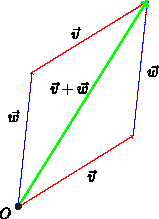
\includegraphics[scale=2.0]{vector_addition.pdf}
   \caption{Vector Addition} 
   \label{fig:figure-2-vector-addition}
\end{figure}

\clearpage

\subsubsection*{Vector Addition Properties}
\vspace{5px}
 
\begin{theorem}[Commutativity]
Suppose $\vec{v}$ and $\vec{w}$ be vectors in $\mathbb{E}^3$.\\
  If $\vec{v} = \left( v_1, v_2, v_3 \right)$ and $\vec{w} = \left(w_1, w_2, w_3 \right)$ be vectors in $\mathbb{E}^{3}$, then
  \begin{equation}
      \vec{v} + \vec{w} = \vec{w} + \vec{v}    
  \end{equation}
\end{theorem}
\begin{proof}
  
\end{proof}


    % end lectures
\end{document}
